\documentclass{article}
\usepackage[left=3cm,top=3cm,right=2cm,bottom=2cm]{geometry}
\usepackage{amssymb}
\usepackage{amsmath}
\usepackage{cancel}
\usepackage[hidelinks]{hyperref}
\usepackage{tikz}

\title{(Universidade de São Paulo)\\
Equações Elípticas}

\author{Métodos Numéricos em Equações Diferenciais\\
Docente: Fabrício Simeoni de Sousa\\[.2cm]
\begin{tabular}{r@{\ }c@{\ }l}
    Kainã Alves Tureso      &-- &15466391\\
    Vinícius de Sá Ferreira &-- &15491650
\end{tabular}}

\date{\today}

\begin{document}
    \maketitle
    
    \section{Problema}
    \begin{align}
        &\frac{\partial^2 u}{\partial x^2}(x,y) + 3\frac{\partial^2 u}{\partial y^2}(x,y) = (4\pi^2-3)\frac{\partial u}{\partial y}(x,y),& (x,y) \in [0,1] \times [-1,1] \label{eq}\\
        &u(0,y)=u(1,y)=0,& y \in [-1,1] \label{dirichlet}\\
        &\frac{\partial u}{\partial \mathbf{n}}(x,-1) = e \sin(2\pi x),\ \frac{\partial u }{\partial \mathbf{n}}(x,1) + u(x,1) = 0,& x \in [0,1] \label{neumann}
    \end{align}

    Em \ref{neumann} temos
    \[\mathbf{n}(x,y) = \begin{pmatrix}0 \\ y\end{pmatrix},\ (x,y) \in [0,1] \times \{-1,1\}\]
    logo
    \[\frac{\partial u}{\partial \mathbf{n}}(x,-1) = e \sin(2\pi x) \iff
    \begin{pmatrix}\frac{\partial u}{\partial x}(x,-1) & \frac{\partial u}{\partial y}(x,-1)\end{pmatrix} \begin{pmatrix}0 \\ -1\end{pmatrix} = e \sin(2\pi x)\]
    \[\iff -\frac{\partial u}{\partial y}(x,-1) = e \sin(2\pi x)\]
    e
    \[\frac{\partial u }{\partial \mathbf{n}}(x,1) + u(x,1) = 0 \iff
    \begin{pmatrix}\frac{\partial u}{\partial x}(x,1) & \frac{\partial u}{\partial y}(x,1)\end{pmatrix} \begin{pmatrix}0 \\ 1\end{pmatrix} + u(x,1) = 0\]
    \[\iff \frac{\partial u}{\partial y}(x,1) + u(x,1) = 0\]

    Portanto, \ref{neumann} pode ser reescrito como
    \begin{align}
        &-\frac{\partial u}{\partial y}(x,-1) = e \sin(2\pi x),\ \frac{\partial u}{\partial y}(x,1) + u(x,1) = 0,& x \in [0,1] \label{neumann_remake}
    \end{align}

    \section{Discretização}
    Usamos os métodos de diferenças finitas centrados para primeira e segunda derivadas, que são $\mathcal{O}(h^2)$
    \[u'(x_n) \approx Du(x_n) = \frac{u(x_{n+1})-u(x_{n-1})}{2h}\]
    \[u''(x_n) \approx D^2u(x_n) = \frac{u(x_{n-1})-2u(x_n)+u(x_{n+1})}{h^2}\]
    Definimos $x_i = ih$ e $y_j = -1 + jh$, com $i \in \{0,1,\cdots,n+1\}$ e $j \in \{0,1,\cdots,m+1\}$, onde $h = \frac{1}{n+1} = \frac{2}{m+1}$. Então o problema se transforma em:
        \begin{align}
        &\frac{U_{i-1,j}-2U_{i,j}+U_{i+1,j}}{h^2} + 3\left(\frac{U_{i,j-1}-2U_{i,j}+U_{i,j+1}}{h^2}\right) = (4\pi^2-3)\frac{U_{i,j+1}-U_{i,j-1}}{2h} \label{num_eq} \begin{array}{l}
            i \in \{1,\cdots,n\}\\
            j \in \{0,\cdots,m+1\}
        \end{array}\\
        &{\color{red}U_{0,j}} = {\color{red}U_{n+1,j}} = 0 \label{num_dirichlet}\qquad j \in \{0,\cdots,m+1\}\\
        &-\left(\frac{U_{i,1}-U_{i,-1}}{2h}\right) = e \sin(2\pi x_i),\ \frac{U_{i,m+2}-U_{i,m}}{2h} + U_{i,m+1} = 0 \label{num_neumann}\qquad i \in \{1,\cdots,n\}
    \end{align}

    Para as condições \ref{num_neumann}, definimos uma série de pontos fantasma $U_{i,-1}$ e $U_{i,m+2}$. Isolando-os, podemos encontrar seus valores em função de pontos da malha e então acrescentar no estêncil do ponto central. Dessa forma, os pontos com condição de Neumann ou Robin são tratados como pontos do interior do domínio, exceto com relação aos pesos atribuídos no estêncil. Assim, simplificamos as expressões acima:
    \begin{align}
        &\frac{1}{h^2}(U_{i-1,j} + U_{i+1,j} - 8 U_{i,j}) + \left(\frac{3}{h^2} + \frac{4\pi^2 -3}{2h}\right)U_{i,j-1} + \left(\frac{3}{h^2} - \frac{4\pi^2 -3}{2h}\right) U_{i,j+1} = 0 \label{simp_eq} \text{\footnotesize $\begin{array}{l}
            i \in \{1,\cdots,n\}\\
            j \in \{0,\cdots,m+1\}
        \end{array}$}\\
        &{\color{red}U_{0,j}} = {\color{red}U_{n+1,j}} = 0 \label{simp_dirichlet}\qquad j \in \{0,\cdots,m+1\}\\
        &U_{i, -1} = U_{i, 1} + 2he\sin(2\pi ih),\ U_{i,m+2} = U_{i,m} - 2h U_{i,m+1} \label{simp_neumann}\qquad i \in \{1,\cdots,n\}
    \end{align}

    \section{Construção do sistema linear}
    As temperaturas de interesse estão no interior e fronteiras verticais (devido à condição de contorno de Neumann), que são definidas na ordem
    \[\mathbf{U} = \begin{pmatrix}
        \color{blue}{U_{1,0}}\\
        \color{blue}{U_{2,0}}\\
        \vdots\\
        \color{blue}{U_{n,0}}\\
        U_{1,1}\\
        \vdots\\
        \color{blue}{U_{1,m+1}}\\
        \vdots\\
        \color{blue}{U_{n,m+1}}
    \end{pmatrix} = \begin{pmatrix}
        \color{blue}{U_1}\\
        \color{blue}{U_2}\\
        \vdots\\
        \color{blue}{U_n}\\
        U_{n+1}\\
        \vdots\\
        \color{blue}{U_{1+n(m+1)}}\\
        \vdots\\
        \color{blue}{U_{n(m+2)}}
    \end{pmatrix} \text{ onde $U_k = U_{i,j},\ k = i + nj$}\]
    \[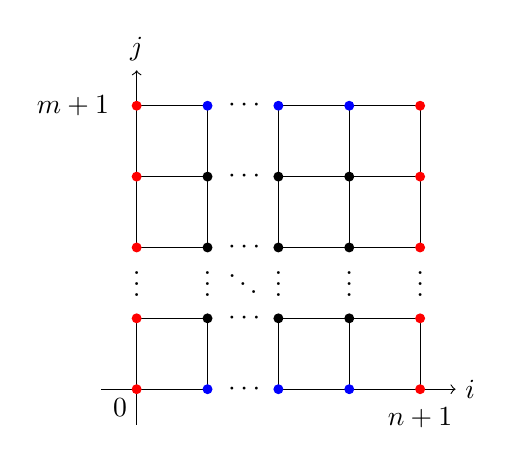
\begin{tikzpicture}[scale=0.9, x=1cm, y=1cm]

        % linhas verticais
        \draw (1,0) -- (1,1); \draw (1,2) -- (1,4);
        \draw (2,0) -- (2,1); \draw (2,2) -- (2,4);
        \draw (3,0) -- (3,1); \draw (3,2) -- (3,4);
        \draw (4,0) -- (4,1); \draw (4,2) -- (4,4);

        % linhas horizontais
        \draw (0,1) -- (1,1); \draw (2,1) -- (4,1);
        \draw (0,2) -- (1,2); \draw (2,2) -- (4,2);
        \draw (0,3) -- (1,3); \draw (2,3) -- (4,3);
        \draw (0,4) -- (1,4); \draw (2,4) -- (4,4);

        % reticências horizontais
        \node at (1.55,0) {$\cdots$};
        \node at (1.55,1) {$\cdots$};
        \node at (1.55,2) {$\cdots$};
        \node at (1.55,3) {$\cdots$};
        \node at (1.55,4) {$\cdots$};

        % reticências verticais
        \node at (0,1.6) {$\vdots$};
        \node at (1,1.6) {$\vdots$};
        \node at (2,1.6) {$\vdots$};
        \node at (3,1.6) {$\vdots$};
        \node at (4,1.6) {$\vdots$};

        % reticências diagonais
        \node at (1.5,1.6) {$\ddots$};

        % eixos
        \draw[-] (-0.5,0) -- (1,0);
        \draw[->] (2,0) -- (4+0.5,0) node[right] {$i$};
        \draw[-] (0,-0.5) -- (0,1);
        \draw[->] (0,2) -- (0,4+0.5) node[above] {$j$};

        % pontos visíveis
        \foreach \i in {1,2,3}
        \foreach \j in {0,4}
            \fill[blue] (\i,\j) circle (2pt);

        \foreach \i in {0,4}
        \foreach \j in {0,1,2,3,4}
            \fill[red] (\i,\j) circle (2pt);

        \foreach \i in {1,2,3}
        \foreach \j in {1,2,3}
            \fill (\i,\j) circle (2pt);


        % rótulos simbólicos
        \node at (4,-0.4) {$n+1$};
        \node at (-0.9,4) {$m+1$};
        \node[below left] at (0,0) {$0$};

    \end{tikzpicture}\]

    \newpage

    Note que, para $i \in \{1,\cdots,n\}$ e $j=0$ em \ref{simp_eq}, temos
    \[\frac{1}{h^2}(U_{i-1,0} + U_{i+1,0} - 8 U_{i,0}) + \left(\frac{3}{h^2} + \frac{4\pi^2 -3}{2h}\right)U_{i,-1} + \left(\frac{3}{h^2} - \frac{4\pi^2 -3}{2h}\right) U_{i,1} = 0\]
    então usamos \ref{simp_neumann} para substituir $U_{i,-1}$
    \[\frac{1}{h^2}(U_{i-1,0} + U_{i+1,0} - 8 U_{i,0}) + \left(\frac{3}{h^2} + \frac{4\pi^2 -3}{2h}\right)\Big(U_{i, 1} + 2he\sin(2\pi ih)\Big) + \left(\frac{3}{h^2} - \frac{4\pi^2 -3}{2h}\right) U_{i,1} = 0\]
    \[\frac{1}{h^2}(U_{i-1,0} + U_{i+1,0} - 8 U_{i,0}) + \frac{6}{h^2} U_{i,1} = -\left(\frac{6}{h} + 4\pi^2 -3\right)e\sin(2\pi ih)\]

    Analogamente, para $i \in \{1,\cdots,n\}$ e $j=m+1$ em \ref{simp_eq}, temos
    \[\frac{1}{h^2}(U_{i-1,m+1} + U_{i+1,m+1} - 8 U_{i,m+1}) + \left(\frac{3}{h^2} + \frac{4\pi^2 -3}{2h}\right)U_{i,m} + \left(\frac{3}{h^2} - \frac{4\pi^2 -3}{2h}\right) U_{i,m+2} = 0\]
    então usamos \ref{simp_neumann} para substituir $U_{i,m+2}$
    \[\frac{1}{h^2}(U_{i-1,m+1} + U_{i+1,m+1} - 8 U_{i,m+1}) + \left(\frac{3}{h^2} + \frac{4\pi^2 -3}{2h}\right)U_{i,m} + \left(\frac{3}{h^2} - \frac{4\pi^2 -3}{2h}\right) \Big(U_{i,m} - 2h U_{i,m+1}\Big) = 0\]
    \[\frac{1}{h^2}(U_{i-1,m+1} + U_{i+1,m+1} - 8 U_{i,m+1}) + \frac{6}{h^2} U_{i,m} + \left(-\frac{6}{h} + 4\pi^2 -3\right) U_{i,m+1} = 0\]
    \[\frac{1}{h^2}(U_{i-1,m+1} + U_{i+1,m+1}) + \left(4\pi^2 -3 -\frac{8}{h^2} - \frac{6}{h}\right)U_{i,m+1} + \frac{6}{h^2} U_{i,m} = 0\]

    Com a notação de $U_k$, a partir de \ref{simp_dirichlet} temos que $U_{nj} = U_{n(j+1)+1} = 0$, logo definimos $U_0 = U_{n(m+2)+1} = 0$. Portanto, para $i \in \{1,\cdots,n\}$ e $j \in \{1,\cdots,m\}$, temos o sistema linear
    \[\begin{cases}
        \displaystyle \frac{1}{h^2}(U_{i-1} + U_{i+1} - 8 U_{i}) + \frac{6}{h^2} U_{i+n} = -\left(\frac{6}{h} + 4\pi^2 -3\right)e\sin(2\pi ih)\\[.5cm]
        \resizebox{0.95\textwidth}{!}{$\displaystyle \frac{1}{h^2}(U_{i-1+nj} + U_{i+1+nj} - 8 U_{i+nj}) + \left(\frac{3}{h^2} + \frac{4\pi^2 -3}{2h}\right)U_{i+n(j-1)} + \left(\frac{3}{h^2} - \frac{4\pi^2 -3}{2h}\right) U_{i+n(j+1)} = 0$}\\[.5cm]
        \displaystyle \frac{1}{h^2}(U_{i-1+n(m+1)} + U_{i+1+n(m+1)}) + \left(4\pi^2 -3 -\frac{8}{h^2} - \frac{6}{h}\right)U_{i+n(m+1)} + \frac{6}{h^2} U_{i+nm} = 0
    \end{cases}\]

    \subsection{Forma matricial}
    Defina as funções
    \[\alpha(h) = \frac{3}{h^2}+\frac{4\pi^2 - 3}{2h},\ \beta(h) = \frac{3}{h^2}-\frac{4\pi^2 - 3}{2h}\]
    
    O sistema linear $M \mathbf{U} = \mathbf{F}$ tem $M$ definido por
    \[M = (A_{-n} + D_{-1} + D_0 + D_{+1} + B_{+n}) + (P_{-n}+Q_{+n}) + G_0\]
    onde
    \[(A_{-n})_{i,j} = \begin{cases}
        \displaystyle \alpha(h), \text{ se $j = i-n$}\\[.2cm]
        0, \text{ caso contrário}
    \end{cases}, (B_{+n})_{i,j} = \begin{cases}
        \displaystyle \beta(h), \text{ se $j = i+n$}\\[.2cm]
        0, \text{ caso contrário}
    \end{cases}\]
    \[(D_{-1})_{i,j} = \begin{cases}
        \displaystyle \frac{1}{h^2}, \text{ se $i\ (\operatorname{mod}\ n) \neq 1$ e $j = i-1$}\\[.2cm]
        0, \text{ caso contrário}
    \end{cases}, (D_{+1})_{i,j} = \begin{cases}
        \displaystyle \frac{1}{h^2}, \text{ se $i\ (\operatorname{mod}\ n) \neq 0$ e $j = i+1$}\\[.2cm]
        0, \text{ caso contrário}
    \end{cases}\]
    \[(D_{0})_{i,j} = \begin{cases}
        \displaystyle -\frac{8}{h^2}, \text{ se $j = i$}\\[.2cm]
        0, \text{ caso contrário}
    \end{cases}\]
    \[(P_{-n})_{i,j} = \begin{cases}
        \displaystyle \beta(h), \text{ se $j = i-n$ e $i > n(m+1)$}\\[.2cm]
        0, \text{ caso contrário}
    \end{cases}, (Q_{+n})_{i,j} = \begin{cases}
        \displaystyle \alpha(h), \text{ se $j = i+n$ e $i \leq n$}\\[.2cm]
        0, \text{ caso contrário}
    \end{cases}\]
    \[(G_0)_{i,j} = \begin{cases}
        \displaystyle -2h\beta(h), \text{ se $i > n(m+1)$}\\[.2cm]
        0, \text{ caso contrário}
    \end{cases}\]

    Porém, podemos simplificar essa decomposição usando produto de Kronecker
    \[A_{-n} + D_{-1} + D_0 + D_{+1} + B_{+n} = I_{m+2} \otimes T_{n} + I_{n} \otimes T_{m+2}\]
    onde $I_{m+2}$ é a matriz identidade de dimensões $(m+2) \times (m+2)$, $I_n$ é a identidade $n \times n$ e
    \[T_n = \begin{pmatrix}
        -\frac{4}{h^2} & \frac{1}{h^2} & 0 & \cdots & 0 \\[.2cm]
        \frac{1}{h^2} & -\frac{4}{h^2} & \frac{1}{h^2} & \cdots & 0 \\[.2cm]
        0 & \frac{1}{h^2} & -\frac{4}{h^2} & \ddots & \vdots \\[.2cm]
        \vdots & \ddots & \ddots & \ddots & \frac{1}{h^2} \\[.2cm]
        0 & \cdots & 0 & \frac{1}{h^2} & -\frac{4}{h^2}
    \end{pmatrix}_{n \times n} \text{ e } T_{m+2} = \begin{pmatrix}
        -\frac{4}{h^2} & \beta(h) & 0 & \cdots & 0 \\[.2cm]
        \alpha(h) & -\frac{4}{h^2} & \beta(h) & \cdots & 0 \\[.2cm]
        0 & \alpha(h) & -\frac{4}{h^2} & \ddots & \vdots \\[.2cm]
        \vdots & \ddots & \ddots & \ddots & \beta(h) \\[.2cm]
        0 & \cdots & 0 & \alpha(h) & -\frac{4}{h^2}
    \end{pmatrix}_{(m+2) \times (m+2)}\]

    Portanto $M = (I_{m+2} \otimes T_{n} + I_{n} \otimes T_{m+2}) + (P_{-n}+Q_{+n}) + G_0$. Temos $\mathbf{U} = \begin{pmatrix}
        U_1\\
        U_2\\
        \vdots\\
        U_{n(m+2)}
    \end{pmatrix}$ como nosso vetor de incógnitas e $\mathbf{F}$ definido por
    \[(F)_{i} = \begin{cases}
        \displaystyle -\left(\frac{6}{h} + 4\pi^2 -3\right)e\sin(2\pi ih), \text{ se $i \leq n$}\\[.2cm]
        0, \text{ caso contrário}
    \end{cases}\]
\end{document}